\documentclass[10pt,a4paper]{article}
\usepackage[utf8]{inputenc}
\usepackage[italian]{babel}
\usepackage{amsmath}
\usepackage{amsfonts}
\usepackage{amssymb}
\usepackage{graphicx}
\usepackage{color}


\title{Promemoria sulle funzioni iperboliche}
\author{Giulio Pasqualetti}
\date{7 febbraio 2015}

\begin{document}

\maketitle

\section{Definizione}

L'unica cosa veramente importante da ricordarsi è la definizione:
\begin{equation}
  \label{eq:definizione}
  \sinh{x} \equiv \frac{e^x-e^{-x}}{2}
  \cosh{x} \equiv \frac{e^x+e^{-x}}{2}
\end{equation}

\section{Grafico e punto di intersezione}

\begin{figure}
  \centering
  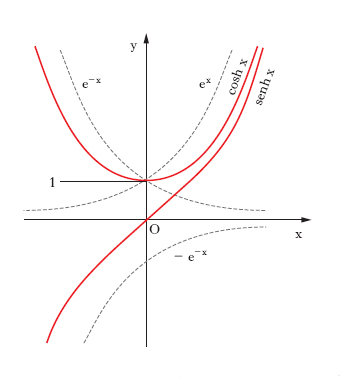
\includegraphics[width=8cm]{./funzioni_iperboliche.jpg}
  \caption{Grafico delle funzioni iperboliche}
  \label{fig:grap}
\end{figure}
Ci sono punti di intersezione tra $\sinh{x}$ e $\cosh{x}$?
\begin{align*}
  \sinh{x} - \cosh{x} &= 0\\
  e^{x}-e^{-x} - e^{x} - e^{-x} &= 0 \\
  2 e^{-x} &= 0
\end{align*}
E quindi non ci sono punti di intersezione.  

\section{Identità fondamentale}
\begin{equation}
  \label{eq:identita}
  \cosh{x}^2 - sinh{x}^2 = 1
\end{equation}

\section{Tangente iperbolica}

\begin{align*}
  \tanh{x} &= \frac{e^x - e^{-x}}{e^x + e^{-x}} \\
  &= \frac{e^{2x}-1}{e^{2x}+1}
\end{align*}

\section{Derivate}

\begin{align*}
  \frac{\mathrm d}{\mathrm d x}\sinh{x} &= \cosh{x} \\
  \frac{\mathrm d}{\mathrm d x}\cosh{x} &= \sinh{x} \\
  \frac{\mathrm d}{\mathrm d x}\tanh{x} &= \frac{\cosh{x}^2-\sinh{x}^2}{\cosh{x}^2}= \frac{1}{\cosh{x}^2}
\end{align*}

\section{Funzioni inverse}

\subsection{$\operatorname{arsinh}{x}$}
\begin{align*}
 y &= \frac{e^x-e^{-x}}{2} \\
e^{2x} -2y e^x -1 &=0 \\
e^x &= y \pm \sqrt{y^2+1} \\
x &= \ln{\big(y + \sqrt{y^2+1}\big)} \\
\operatorname{arsinh}{x} &= \ln{\big(x +  \sqrt{x^2 + 1}\big)}
\end{align*}

\section{Sviluppo in serie}

\begin{equation}
  \label{eq:taylor_sinhx}
  \sinh{x} = x + \frac{x^3}{3!} + \mathrm{O}(x^5)
\end{equation}
\begin{equation}
  \label{eq:taylor_coshx}
  \cosh{x} = 1 + \frac{x^2}{2} + \mathrm{O}(x^4)
\end{equation}
\end{document}